%1-lep DNN ML
\clearpage
\section{Fit Results with Unblinded Data}
\label{sec:Fit_Results_ub}

Using the methodology detailed in earlier sections of this chapter, we have obtained promising unblinded results using the DNN. 
Table~\ref{tab:significance_1lepdnn} presents both expected and observed significances for the \olep channel. The expected significance is derived from Asimov data, with adjustments for background normalization and nuisance parameters. 
Remarkably, the observed significance from actual data surpasses the critical 5$\sigma$ threshold. This achievement marks the first time we reach this level of significance in the semileptonic final states for electroweak $VV+jj$ production within a VBS-enhanced phase space, using only the \olep channel.
We observe a deficit compared to the expected significance. Although the DNN fitting approach does not account for certain signal uncertainties, such as EWK-QCD interference and shower systematics, the results are robust enough to serve as a corroborative cross-check against other baseline analyses using different ML approaches.


\begin{table}[h]
  \centering
  \begin{tabular}{|c|c|}
    \hline
           & 1-lep \\
    \hline
    Expected pre-fit significance & 5.39 \\
    \hline
    Expected post-fit significance & 5.98 \\
    \hline
    Observed significance & 5.78 \\
    \hline
  \end{tabular}
  \caption{Expected and observed significances for the \olep channel.}
  \label{tab:significance_1lepdnn}
\end{table}

Preliminary DNN fitting yields a signal strength parameter $\mu_{VBS} = 1.16 \pm 0.25$. 
Table~\ref{tab:break_1lepdnn} shows the uncertainty breakdown on $\mu_{VBS}$ for the \olep channel.
Postfit distributions for the SRs with full range data are shown in Figure~\ref{fig:postfitsr_1lepdnn}, while the corresponding distributions for the CRs are displayed in Figure~\ref{fig:postfitcr_1lepdnn}. These distributions demonstrate satisfactory agreement between the data and the MC simulations.
Tables~\ref{tab:1lepPostfitYield_SR}-\ref{tab:1lepPostfitYield_CR} show the postfit event yields for signal and background processes in all the CRs and SRs.

\begin{figure}[h]
  \centering
  \subfloat[Merged HP]{
    \includegraphics[width=.32\textwidth]{figures/FitResults/postfit/Region_distDNN_DSRVBSHP_BMin0_J0_incJet1_L1_T0_incFat1_Y6051_incTag1_Fat1_GlobalFit_unconditionnal_mu1log.pdf}
  }
  \subfloat[Merged LP]{
    \includegraphics[width=.32\textwidth]{figures/FitResults/postfit/Region_distDNN_DSRVBSLP_BMin0_J0_incJet1_L1_T0_incFat1_Y6051_incTag1_Fat1_GlobalFit_unconditionnal_mu1log.pdf}
  }
  \subfloat[Resolved]{
    \includegraphics[width=.32\textwidth]{figures/FitResults/postfit/Region_distDNN_DSRVBSTight_BMin0_T0_Y6051_incTag1_J2_L1_incJet1_GlobalFit_unconditionnal_mu1log.pdf}
  }
  \caption{Postfit plots for SR distributions}
  \label{fig:postfitsr_1lepdnn}
\end{figure}

\begin{figure}[h]
  \centering

  \subfloat[Resolved Top CR]{
    \includegraphics[width=.32\textwidth]{figures/FitResults/postfit/Region_disttagMjj_DCRTopTight_BMin0_T0_Y6051_incTag1_J2_L1_incJet1_GlobalFit_unconditionnal_mu1log.pdf}
  }
  \subfloat[Resolved Wjet CR]{
    \includegraphics[width=.32\textwidth]{figures/FitResults/postfit/Region_disttagMjj_DCRVjetTight_BMin0_T0_Y6051_incTag1_J2_L1_incJet1_GlobalFit_unconditionnal_mu1log.pdf}
  }
  \subfloat[Merged Wjet CR]{
    \includegraphics[width=.32\textwidth]{figures/FitResults/postfit/Region_disttagMjj_DCRVjetMerged_BMin0_J0_incJet1_L1_T0_incFat1_Y6051_incTag1_Fat1_GlobalFit_unconditionnal_mu1log.pdf}
  }

  \subfloat[Merged LP Top CR]{
    \includegraphics[width=.32\textwidth]{figures/FitResults/postfit/Region_disttagMjj_DCRTopLP_BMin0_J0_incJet1_L1_T0_incFat1_Y6051_incTag1_Fat1_GlobalFit_unconditionnal_mu1.pdf}
  }
  \subfloat[Merged HP Top CR]{
    \includegraphics[width=.32\textwidth]{figures/FitResults/postfit/Region_disttagMjj_DCRTopHP_BMin0_J0_incJet1_L1_T0_incFat1_Y6051_incTag1_Fat1_GlobalFit_unconditionnal_mu1.pdf}
  }

  \caption{Postfit plots for CR distributions}
  \label{fig:postfitcr_1lepdnn}
\end{figure}

\begin{table}[h]
\centering
\begin{tabular}{|l|c|c|c|}
\hline
Uncertainty Source & Positive Error & Negative Error & Symmetric Uncertainty \\
\hline
Total                    & \(+0.263\) & \(-0.237\) & \(\pm 0.250\) \\
DataStat                 & \(+0.107\) & \(-0.105\) & \(\pm 0.106\) \\
FullSyst                 & \(+0.240\) & \(-0.212\) & \(\pm 0.226\) \\
\hline
Floating normalizations  & \(+0.044\) & \(-0.035\) & \(\pm 0.039\) \\
All normalizations       & \(+0.095\) & \(-0.079\) & \(\pm 0.087\) \\
All but normalizations   & \(+0.230\) & \(-0.202\) & \(\pm 0.216\) \\
Jets MET                 & \(+0.132\) & \(-0.118\) & \(\pm 0.125\) \\
BTag                     & \(+0.031\) & \(-0.031\) & \(\pm 0.031\) \\
Leptons                  & \(+0.000\) & \(-0.000\) & \(\pm 0.000\) \\
Luminosity               & \(+0.025\) & \(-0.019\) & \(\pm 0.022\) \\
Diboson                  & \(+0.036\) & \(-0.032\) & \(\pm 0.034\) \\
Model                    & \(+0.148\) & \(-0.128\) & \(\pm 0.138\) \\
Signal Systematics       & \(+0.166\) & \(-0.133\) & \(\pm 0.150\) \\
Mjj reweighting          & \(+0.023\) & \(-0.037\) & \(\pm 0.030\) \\
Quark gluon              & \(+0.015\) & \(-0.009\) & \(\pm 0.012\) \\
MC stat                  & \(+0.082\) & \(-0.077\) & \(\pm 0.079\) \\
\hline
\end{tabular}
\caption{Uncertainty breakdown on $\mu_{VBS}$ in \olep DNN.}
\label{tab:break_1lepdnn}
\end{table}

%%%%%%%postfit_table
% \newcolumntype{d}{D{+}{\hspace{-3pt}\;\pm\;}{-1}}
\documentclass{article}
\usepackage{graphicx}
\newcommand{\GeV}{\mathrm{GeV}}
\newcommand{\ptv}{p_T^V}
\begin{document}
\begin{table}
\centering
\small
\begin{tabular}{l|c|}
\cline{2-2}
 & \multicolumn{1}{c|}{Region\_distDNN\_DSRVBSHP\_BMin0\_J0\_incJet1\_L1\_T0\_incFat1\_Y6051\_incTag1\_Fat1}\\
\cline{2-2}
 & \multicolumn{1}{c|}{Region\_distDNN\_DSRVBSHP\_BMin0\_J0\_incJet1\_L1\_T0\_incFat1\_Y6051\_incTag1\_Fat1}\\ \hline
W & 3772.48 $\pm$ 207.54\\
Z & 175.98 $\pm$ 24.93\\
Diboson & 574.86 $\pm$ 163.38\\
stop & 598.20 $\pm$ 167.59\\
ttbar & 6748.42 $\pm$ 277.01\\
\hline
Bkg & 11869.94 $\pm$ 110.89\\
\hline
EW6lvqq & 239.21 $\pm$ 42.47\\
\hline
Signal & 239.21 $\pm$ 42.47\\
SignalExpected & 206.48 $\pm$ 36.66\\
\hline
S/B & 2.02e-02\\
S/sqrt(S+B) & 2.17e+00\\
\hline
data & 12178\\ \hline
\end{tabular}
\end{table}


\begin{table}
\centering
\small
\begin{tabular}{l|c|}
\cline{2-2}
 & \multicolumn{1}{c|}{Region\_distDNN\_DSRVBSLP\_BMin0\_J0\_incJet1\_L1\_T0\_incFat1\_Y6051\_incTag1\_Fat1}\\
\cline{2-2}
 & \multicolumn{1}{c|}{Region\_distDNN\_DSRVBSLP\_BMin0\_J0\_incJet1\_L1\_T0\_incFat1\_Y6051\_incTag1\_Fat1}\\ \hline
W & 10111.99 $\pm$ 371.67\\
Z & 462.53 $\pm$ 58.40\\
Diboson & 804.42 $\pm$ 231.65\\
stop & 846.84 $\pm$ 244.44\\
ttbar & 9856.21 $\pm$ 356.81\\
\hline
Bkg & 22082.00 $\pm$ 171.45\\
\hline
EW6lvqq & 195.86 $\pm$ 43.72\\
\hline
Signal & 195.86 $\pm$ 43.72\\
SignalExpected & 169.06 $\pm$ 37.74\\
\hline
S/B & 8.87e-03\\
S/sqrt(S+B) & 1.31e+00\\
\hline
data & 22158\\ \hline
\end{tabular}
\end{table}


\begin{table}
\centering
\small
\begin{tabular}{l|c|}
\cline{2-2}
 & \multicolumn{1}{c|}{Region\_distDNN\_DSRVBSTight\_BMin0\_T0\_Y6051\_incTag1\_J2\_L1\_incJet1}\\
\cline{2-2}
 & \multicolumn{1}{c|}{Region\_distDNN\_DSRVBSTight\_BMin0\_T0\_Y6051\_incTag1\_J2\_L1\_incJet1}\\ \hline
W & 57446.51 $\pm$ 785.36\\
Z & 2168.91 $\pm$ 324.79\\
Diboson & 1721.91 $\pm$ 552.18\\
stop & 1521.92 $\pm$ 416.17\\
ttbar & 7633.82 $\pm$ 382.92\\
\hline
Bkg & 70493.07 $\pm$ 317.65\\
\hline
EW6lvqq & 742.72 $\pm$ 133.71\\
\hline
Signal & 742.72 $\pm$ 133.71\\
SignalExpected & 641.09 $\pm$ 115.41\\
\hline
S/B & 1.05e-02\\
S/sqrt(S+B) & 2.78e+00\\
\hline
data & 71272\\ \hline
\end{tabular}
\end{table}


\begin{table}
\centering
\small
\begin{tabular}{l|c|}
\cline{2-2}
 & \multicolumn{1}{c|}{Region\_disttagMjj\_DCRTopHP\_BMin0\_J0\_incJet1\_L1\_T0\_incFat1\_Y6051\_incTag1\_Fat1}\\
\cline{2-2}
 & \multicolumn{1}{c|}{Region\_disttagMjj\_DCRTopHP\_BMin0\_J0\_incJet1\_L1\_T0\_incFat1\_Y6051\_incTag1\_Fat1}\\ \hline
W & 279.58 $\pm$ 16.61\\
Z & 18.94 $\pm$ 2.83\\
Diboson & 46.59 $\pm$ 13.86\\
stop & 1113.16 $\pm$ 307.91\\
ttbar & 10728.53 $\pm$ 343.94\\
\hline
Bkg & 12186.80 $\pm$ 109.43\\
\hline
EW6lvqq & 74.71 $\pm$ 14.77\\
\hline
Signal & 74.71 $\pm$ 14.77\\
SignalExpected & 64.48 $\pm$ 12.75\\
\hline
S/B & 6.13e-03\\
S/sqrt(S+B) & 6.75e-01\\
\hline
data & 12195\\ \hline
\end{tabular}
\end{table}


\begin{table}
\centering
\small
\begin{tabular}{l|c|}
\cline{2-2}
 & \multicolumn{1}{c|}{Region\_disttagMjj\_DCRTopLP\_BMin0\_J0\_incJet1\_L1\_T0\_incFat1\_Y6051\_incTag1\_Fat1}\\
\cline{2-2}
 & \multicolumn{1}{c|}{Region\_disttagMjj\_DCRTopLP\_BMin0\_J0\_incJet1\_L1\_T0\_incFat1\_Y6051\_incTag1\_Fat1}\\ \hline
W & 717.29 $\pm$ 36.10\\
Z & 47.45 $\pm$ 6.56\\
Diboson & 68.76 $\pm$ 19.33\\
stop & 1227.37 $\pm$ 363.11\\
ttbar & 15013.46 $\pm$ 390.23\\
\hline
Bkg & 17074.34 $\pm$ 212.66\\
\hline
EW6lvqq & 63.89 $\pm$ 14.29\\
\hline
Signal & 63.89 $\pm$ 14.29\\
SignalExpected & 55.15 $\pm$ 12.33\\
\hline
S/B & 3.74e-03\\
S/sqrt(S+B) & 4.88e-01\\
\hline
data & 17195\\ \hline
\end{tabular}
\end{table}


\clearpage


\begin{table}
\centering
\small
\begin{tabular}{l|c|}
\cline{2-2}
 & \multicolumn{1}{c|}{Region\_disttagMjj\_DCRTopTight\_BMin0\_T0\_Y6051\_incTag1\_J2\_L1\_incJet1}\\
\cline{2-2}
 & \multicolumn{1}{c|}{Region\_disttagMjj\_DCRTopTight\_BMin0\_T0\_Y6051\_incTag1\_J2\_L1\_incJet1}\\ \hline
W & 2044.50 $\pm$ 71.00\\
Z & 101.67 $\pm$ 15.16\\
Diboson & 81.79 $\pm$ 26.43\\
stop & 1885.19 $\pm$ 514.80\\
ttbar & 11853.62 $\pm$ 565.44\\
\hline
Bkg & 15966.76 $\pm$ 138.04\\
\hline
EW6lvqq & 155.57 $\pm$ 31.27\\
\hline
Signal & 155.57 $\pm$ 31.27\\
SignalExpected & 134.28 $\pm$ 26.99\\
\hline
S/B & 9.74e-03\\
S/sqrt(S+B) & 1.23e+00\\
\hline
data & 16137\\ \hline
\end{tabular}
\end{table}


\begin{table}
\centering
\small
\begin{tabular}{l|c|}
\cline{2-2}
 & \multicolumn{1}{c|}{Region\_disttagMjj\_DCRVjetMerged\_BMin0\_J0\_incJet1\_L1\_T0\_incFat1\_Y6051\_incTag1\_Fat1}\\
\cline{2-2}
 & \multicolumn{1}{c|}{Region\_disttagMjj\_DCRVjetMerged\_BMin0\_J0\_incJet1\_L1\_T0\_incFat1\_Y6051\_incTag1\_Fat1}\\ \hline
W & 22644.17 $\pm$ 842.49\\
Z & 1147.58 $\pm$ 146.40\\
Diboson & 1225.46 $\pm$ 347.60\\
stop & 1294.60 $\pm$ 360.16\\
ttbar & 11995.36 $\pm$ 787.80\\
\hline
Bkg & 38307.18 $\pm$ 211.01\\
\hline
EW6lvqq & 124.40 $\pm$ 23.18\\
\hline
Signal & 124.40 $\pm$ 23.18\\
SignalExpected & 107.37 $\pm$ 20.01\\
\hline
S/B & 3.25e-03\\
S/sqrt(S+B) & 6.35e-01\\
\hline
data & 38486\\ \hline
\end{tabular}
\end{table}


\begin{table}
\centering
\small
\begin{tabular}{l|c|}
\cline{2-2}
 & \multicolumn{1}{c|}{Region\_disttagMjj\_DCRVjetTight\_BMin0\_T0\_Y6051\_incTag1\_J2\_L1\_incJet1}\\
\cline{2-2}
 & \multicolumn{1}{c|}{Region\_disttagMjj\_DCRVjetTight\_BMin0\_T0\_Y6051\_incTag1\_J2\_L1\_incJet1}\\ \hline
W & 501272.25 $\pm$ 9637.60\\
Z & 21630.23 $\pm$ 3315.37\\
Diboson & 15241.39 $\pm$ 4878.27\\
stop & 29343.00 $\pm$ 8099.30\\
ttbar & 231974.93 $\pm$ 10369.58\\
\hline
Bkg & 799461.79 $\pm$ 2665.92\\
\hline
EW6lvqq & 1989.35 $\pm$ 394.05\\
\hline
Signal & 1989.35 $\pm$ 394.05\\
SignalExpected & 1717.15 $\pm$ 340.13\\
\hline
S/B & 2.49e-03\\
S/sqrt(S+B) & 2.22e+00\\
\hline
data & 801406\\ \hline
\end{tabular}
\end{table}


\end{document}



Figure~\ref{fig:fit_1lep_corr_all_data} shows the correlation matrix for the full-range data fit. 
Figures~\ref{fig:fit_1lep_fcc_data}-\ref{fig:fit_1lep_ranking_all_data} display the pulls of the NPs and the ranking plots for the unblinded full-range data fit. 
The leading uncertainties impacting the fit include the theoretical QCD uncertainty on the signal, the modeling uncertainties of the \Wjets background, the reweighting uncertainties of the tagging jets, and \texttt{SysJET\_JERComb}, the baseline uncertainties from the small-$R$ jets resolution.

\begin{figure}[ht]
      \centering
        \includegraphics[width=\linewidth]{figures/Fit_fcc/GlobalFit/corr_HighCorrNoMCStat.pdf}
        \caption{Correlations for unconditional fit ($\mu=1$) to unblinded data in the full range.}
       \label{fig:fit_1lep_corr_all_data}
\end{figure}

\begin{figure}[ht]
      \centering
        \includegraphics[width=\linewidth]{figures/Fit_fcc/GlobalFit/NP_allExceptGammas.pdf}
        \caption{Fit cross-check, the pulls of the NPs for the unblinded fit.}
       \label{fig:fit_1lep_fcc_data}
\end{figure}

\begin{figure}[ht]
      \centering
        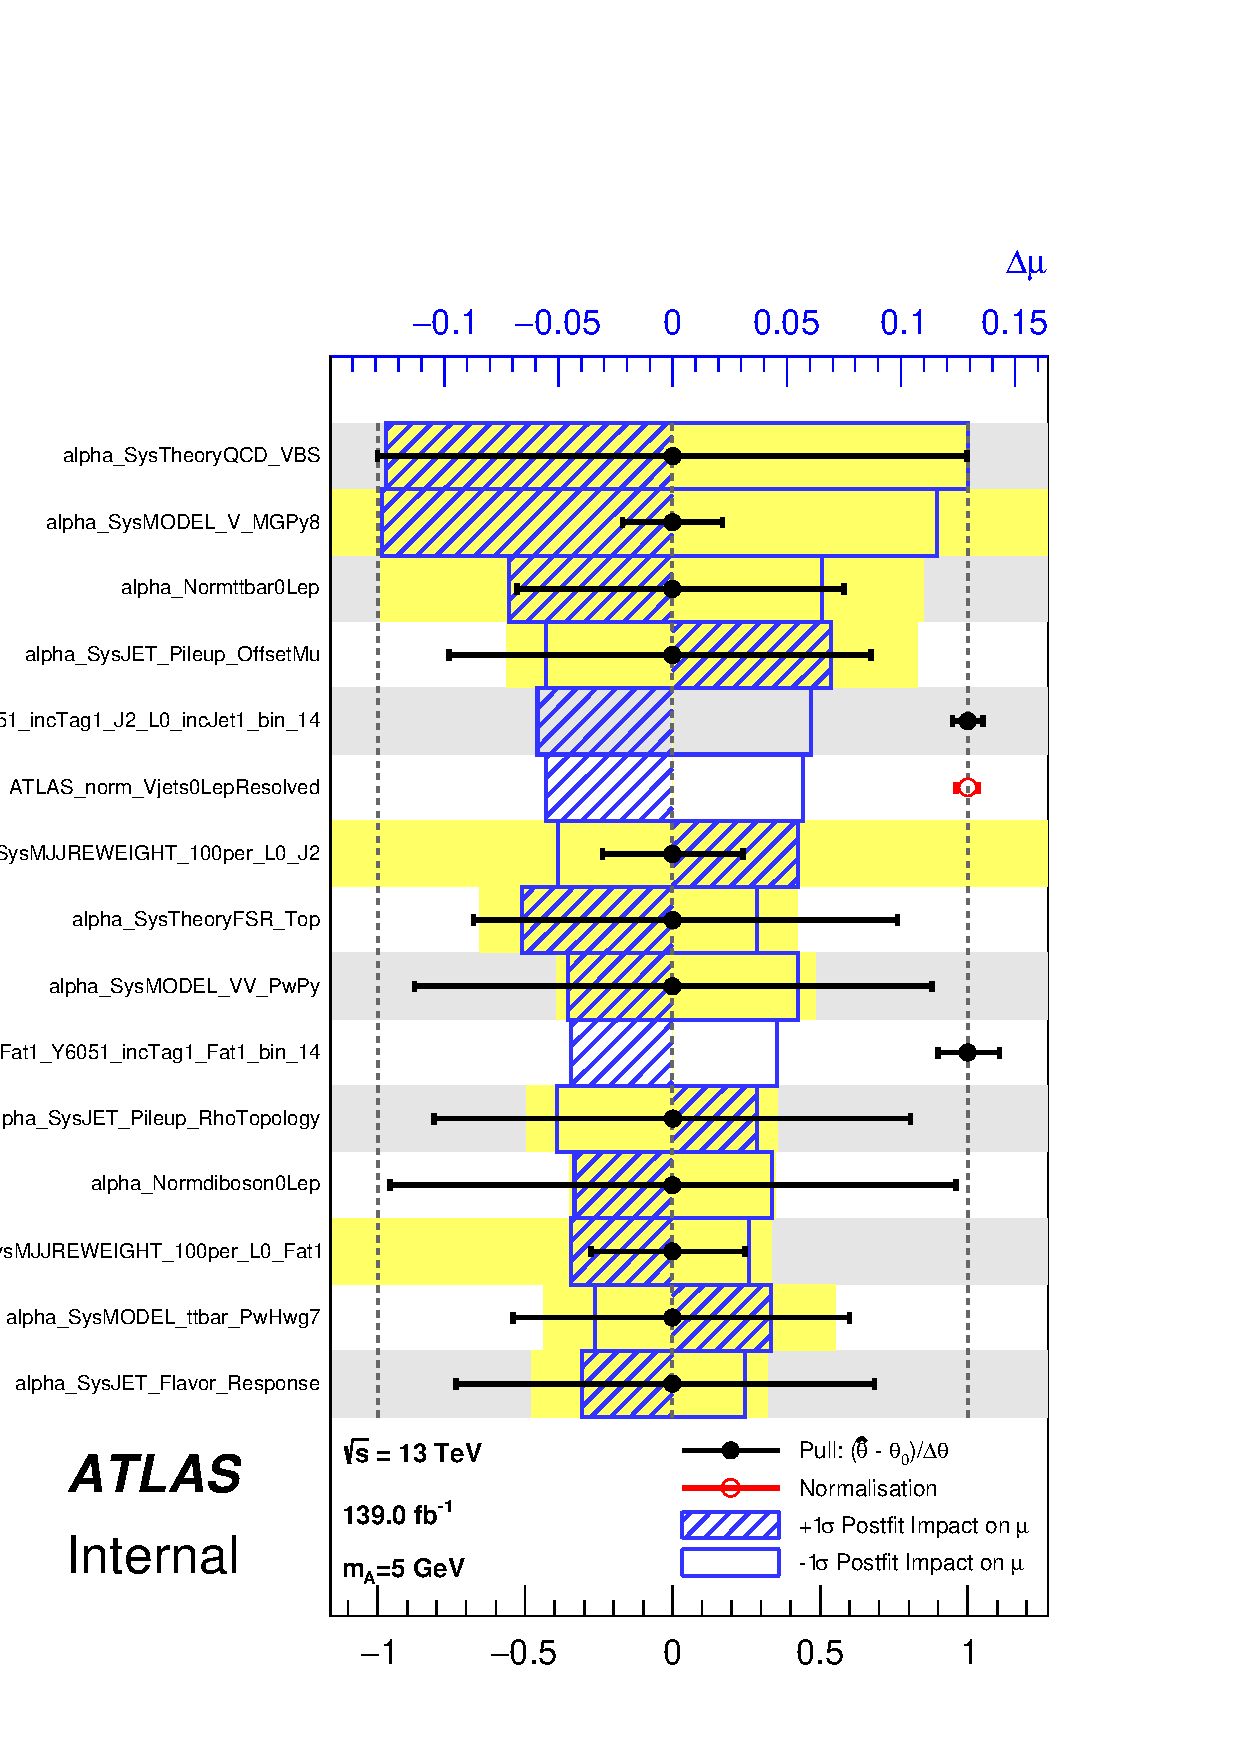
\includegraphics[width=0.5\textwidth]{figures/Fit_np_rank/pulls_mu_Global/pulls_mu_SemileptonicVBS_5.pdf}
        \caption{Ranking of nuisance parameters postfit-sorted for the unblinded fit.}
       \label{fig:fit_1lep_ranking_all_data}
\end{figure}


